\section{Section}\label{sse:Section}

\subsection{Subsection}\label{sss:Subsection}

Subsection \ref{sss:Subsection} contains Equation \eqref{eq:convection-diffusion}:

\begin{equation}\label{eq:convection-diffusion}
    \frac{\p c}{\p t} - D \Delta c + \mathbfit{v}\cdot\nabla c = f.
\end{equation}

Example citation \citep{baarslag2015learning}

\dfn{Title}{dfn_ref}{Definition environment.}

Reference to Definition \ref{dfn:dfn_ref}.

\qs{Title}{qs_ref}{Question environment.}

\sol{Solution to Question \ref{qs:qs_ref}}.

\clm{Title}{clm_ref}{Claim environment.}

Reference to Claim \ref{clm:clm_ref}

\ex{Title}{ex_ref}{Example environment.}

Reference to Example \ref{ex:ex_ref}.

\thm{Title}{thm_ref}{Theorem environment.}

\pf{of Theorem \ref{thm:thm_ref}}{Proof environment.}

\cor{Title}{cor_ref}{Corollary environment.}

Reference to Corollary \ref{cor:cor_ref}.

\lem{Title}{lem_ref}{Lemma environment.}

Reference to Lemma \ref{lem:lem_ref}.

\prp{Title}{prp_ref}{Proposition environment.}

Reference to Proposition \ref{prp:prp_ref}.

\begin{figure}[H]
    \centering
    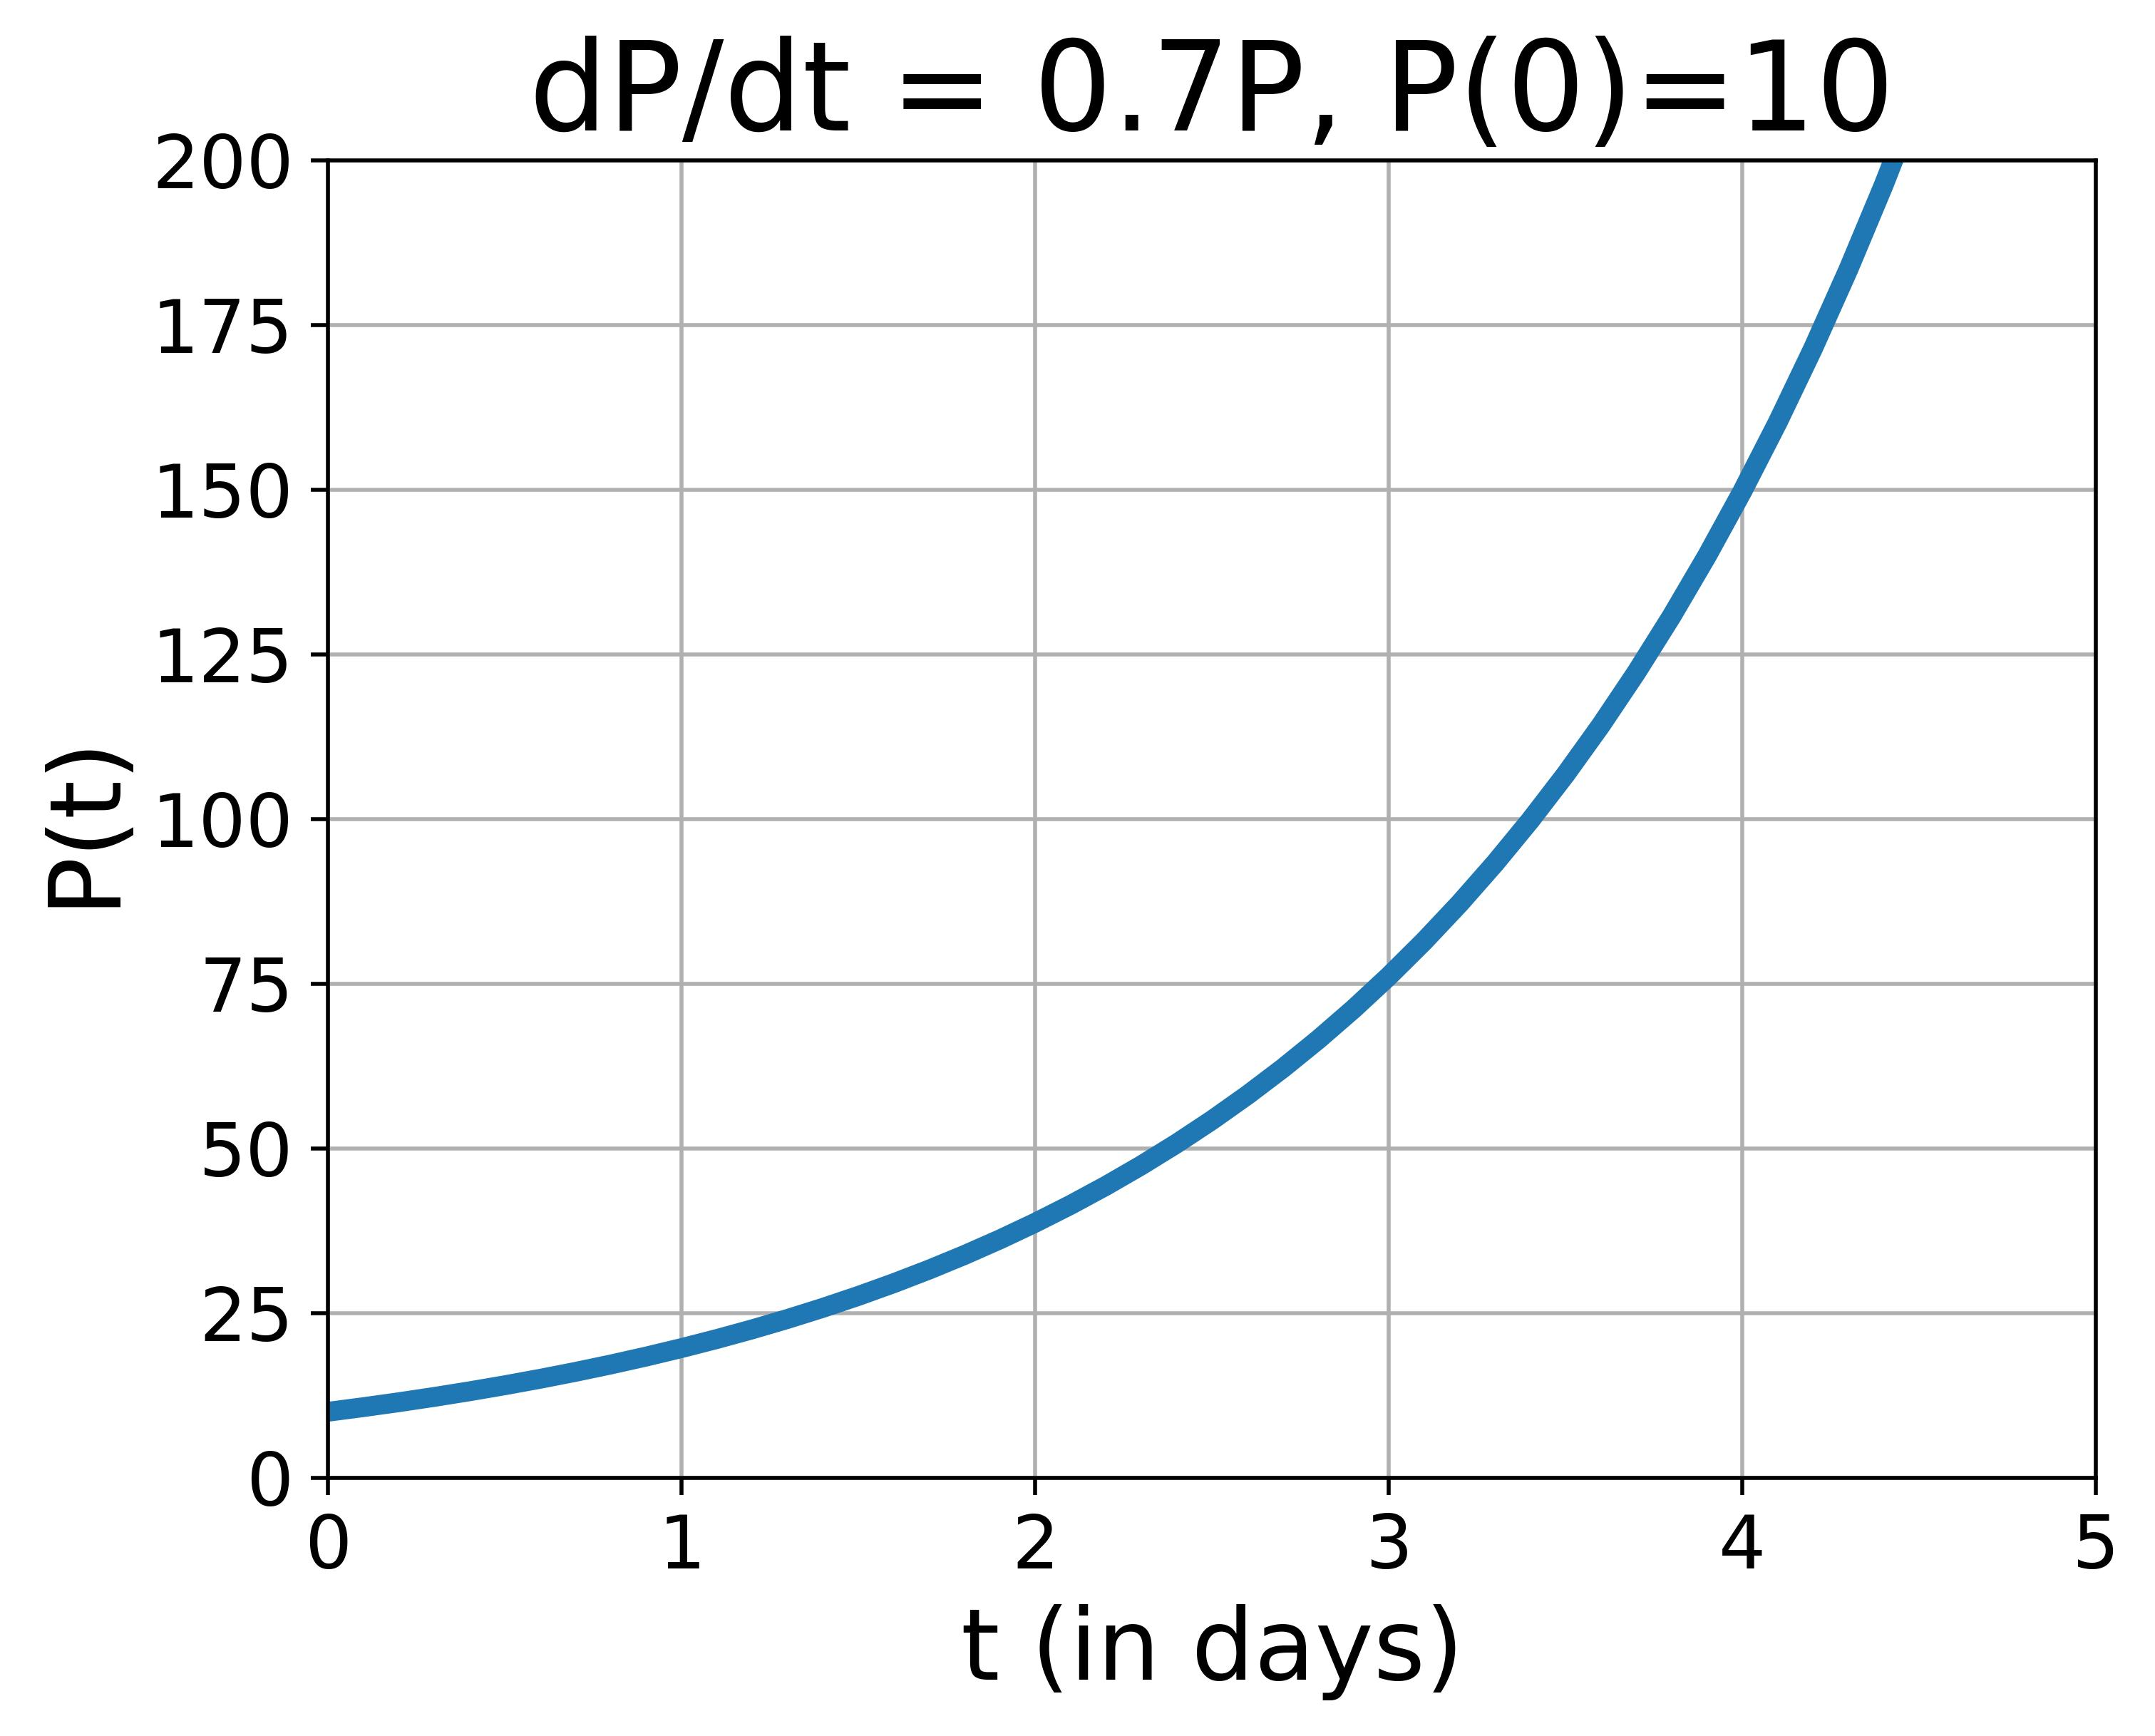
\includegraphics[width=0.5\textwidth]{Rainbowfish.jpg}
    \caption[Rainbowfish population as a function of time]{Rainbowfish population as a function of time \citep{tudelftopencourseware}.}
    \label{fig:Rainbowfish}
\end{figure}

\begin{table}[H]
    \centering
    \resizebox{0.28\textwidth}{!}{%
        \begin{tabular}{c|c}
            Time (day) & Population (-) \\
            \hline
            0.00       & 10.00          \\
            1.00       & 19.67          \\
            2.00       & 38.70          \\
            3.00       & 76.12          \\
            4.00       & 149.74         \\
            5.00       & 294.57
        \end{tabular}%
    }
    \caption[Rainbowfish population as a function of time]{Rainbowfish population as a function of time \citep{tudelftopencourseware}.}
    \label{tab:ohno}
\end{table}